\documentclass[onecolumn, draftclsnofoot,10pt, compsoc]{IEEEtran}
\usepackage{graphicx}
\usepackage{url}
\usepackage{setspace}
\usepackage{graphicx}
\usepackage{epstopdf}
\usepackage{float}

\usepackage{geometry}
\geometry{textheight=9.5in, textwidth=7in}

% 1. Fill in these details
\def \CapstoneTeamName{		Team TriTone}
\def \CapstoneTeamNumber{		045}
\def \GroupMemberOne{			Aidan O'Malley}
\def \GroupMemberTwo{			Christopher Hebert}
\def \GroupMemberThree{			Kazuriah Buckley}
\def \CapstoneProjectName{		Music Theory Application}
\def \CapstoneSponsorPerson{		Lukas Hein}

% 2. Uncomment the appropriate line below so that the document type works
\def \DocType{		%Problem Statement
				%Requirements Document
				%Technology Review
  Design Document
				%Progress Report
				}
			
\newcommand{\NameSigPair}[1]{\par
\makebox[2.75in][r]{#1} \hfil 	\makebox[3.25in]{\makebox[2.25in]{\hrulefill} \hfill		\makebox[.75in]{\hrulefill}}
\par\vspace{-12pt} \textit{\tiny\noindent
\makebox[2.75in]{} \hfil		\makebox[3.25in]{\makebox[2.25in][r]{Signature} \hfill	\makebox[.75in][r]{Date}}}}
% 3. If the document is not to be signed, uncomment the RENEWcommand below
\renewcommand{\NameSigPair}[1]{#1}

%%%%%%%%%%%%%%%%%%%%%%%%%%%%%%%%%%%%%%%
\begin{document}
\begin{titlepage}
    \pagenumbering{gobble}
    \begin{singlespace}
    	
\includegraphics[height=4cm]{coe_v_spot1}
        \hfill 
        % 4. If you have a logo, use this includegraphics command to put it on the coversheet.
        %\includegraphics[height=4cm]{CompanyLogo}   
        \par\vspace{.2in}
        \centering
        \scshape{
            \huge CS Capstone \DocType \par
            {\large\today}\par
            \vspace{.5in}
            \textbf{\Huge\CapstoneProjectName}\par
            \vfill
            %{\large Prepared for}\par
            %\Huge \CapstoneSponsorCompany\par
            \vspace{5pt}
                   {\Large\NameSigPair{\CapstoneSponsorPerson}\par}
            {\large Prepared by }\par
            Group\CapstoneTeamNumber\par
            % 5. comment out the line below this one if you do not wish to name your team
            \CapstoneTeamName\par 
            \vspace{5pt}
            {\Large
                \NameSigPair{\GroupMemberOne}\par
                \NameSigPair{\GroupMemberTwo}\par
                \NameSigPair{\GroupMemberThree}\par
            }
            \vspace{20pt}
        }
        \begin{abstract}
          The purpose of this document is to outline the system architecture and design decisions made for the Music Theory Application.
          The scope and purpose of the application is summarized.
          The system architecture and implementation language are specified.
          The pages of the application are laid out and their implementations are described.
        \end{abstract}     
    \end{singlespace}
\end{titlepage}
\newpage
\pagenumbering{arabic}
\tableofcontents
% 7. uncomment this (if applicable). Consider adding a page break.
%\listoffigures
%\listoftables
\clearpage

\section{Introduction}
\subsection{Scope}
The piece of software discussed in the following document is intended to be used as an educational resource for musicians of all experience levels. 
Our goal is to create an application that will enhance the quality of musicians around the world by teaching concepts of functional harmony.

\subsection{Purpose}
The purpose of the following software design document is to outline the design of the application at a fairly low level.
All functionality of the application that is necessary in achieving our team’s goals for a completed product are contained in this document.		

\subsection{Intended Audience}
This document is intended for capstone instructors and teaching assistants as well as for our group and client’s reference for the upcoming terms. 
Anyone interested in the development process of the application will also find the following document useful. 
However, this document will mainly be used to define a set of design goals to be used in comparison with our final product.		

\subsection{Conformance}
This document conforms with the requirements outlined by the client, Lukas Hein, during the many meetings conducted between the client and the team over the course of fall term. 
Any changes to design will be reflected in revisions to this document.

\subsection{Definitions and Acronyms}
\begin{itemize}
\item \textbf{COF}: 
  Meaning Circle of Fifths, the main aspect of our application. 
  It is the circle of the 12 tones of western music with the intervals of four going clockwise around and the intervals of five going counter-clockwise.
\item \textbf{Sidebar}:
  The vertical list of the 12 notes in western music that will be placed adjacent to the COF on the application’s main page.
\item \textbf{Composition Page}:
  The page where a user will be able to create their own composition and test their ability to follow the rules of tonal gravity.
\item \textbf{Schedule of Tonal Gravity}:
  The natural direction that a specific note wants to travel when in a specific key.
\item \textbf{Musical Golden Mean}: BEADGCF.
  The tonal gravity of the key of C, from left to right shows the direction that each chord in the key of C wants to travel.
\item \textbf{Tonal Gravity Rules}: 
  The three rules outlined by Lukas for a key’s tonal gravity. 
  1.) Do not go up consecutive steps of the key’s tonal gravity.
  2.) Do not go down the schedule of tonal gravity by more than one step.
  3.) No limit on steps one can skip when travelling up the schedule of tonal gravity.
\item \textbf{Key Signature}:
  The notes that make up a specific key.
\item \textbf{Parallel Key}:
  The key that has the same root note as our initial key, however, is in the opposite mode.
  For example, C major’s relative key is C minor and visa versa.
\item \textbf{Relative Key}:
  The key that contains all of the same notes as our initial key, however, the root note, chord qualities and schedule of tonal gravity differ \cite{omt-keysig}.
  For example, C major’s relative key is A minor.
\item \textbf{Interval}:
  An interval is the distance between two pitches, usually measured as a number of steps on a scale \cite{omt-intervals}.
\item \textbf{Chord Quality}: The name given to a chord based on the intervals between the root and the other notes that make up the chord \cite{omt-triads}.
\end{itemize}

\section{System Architecture}
\subsection{Design}
Since our client requested that our project be a mobile application we needed to decide on some tool for creating it.
During some of the initial meetings with our client it was clear that we would want the application to run on both android and apple mobile devices and we did not want the application to be web based initially.
So moving forward from here we wanted to chose a framework that would make it easy for us to make a product for both platforms.
After considering our options for the system architecture we chose to use a framework called React Native.
Developing in this component based Javascript framework is much like coding in an object oriented framework because it treats each component much like an object.
This allows us to easily select and implement specific components required to create the interface users will be able to interact with our application through. 

In this framework we can structure a hierarchy of components where a page can be the container component such as the Circle of Fifths page.
This component will then be made up of smaller reusable components like the actual COF, the Sidebar, and the buttons.
These inner components can contain components within them as well and our data will flow logically down this hierarchy to the child components.
In short, the application will start at our home page of the Circle of Fifths page which is its own component.
There will also be container components for the Composition page and the References pages.
These will all have unidirectional data flow and will contain similar components that will be reused between them.
For example, the COF component will be shared on the main page and the composition page.
This structuring provides a very logical and readable codebase and will make our team’s lives easier as we progress.

\subsection{Rationale}
Of the framework options we considered for programming our application in, we decided on React since the framework allows us to implement our application for both Apple and Android devices simultaneously and is very developer friendly.
In addition, the power and simplicity of this specific framework would allow us to quickly become familiar with the necessary components needed to design and implement our application.

\section{Component Design}
\subsection{Circle Of Fifths Page}
The Circle of Fifths page is the main page of our application and will demonstrate most of the concepts that we attempt to educate the user on.
It consists of the COF, the sidebar, buttons to add or remove parallel and relative keys, and buttons to travel to reference and composition pages.

\subsubsection{COF}

\setcounter{secnumdepth}{4}
\paragraph{GUI Design}
From a design viewpoint, the graphical user interface for the main circle will consist of a pie chart that has all of the 12 notes with placement corresponding to the 12 wedges of the pie chart.
The keys will be represented by the key’s chord qualities.
The chart will contain concentric rings to split up the relative key, current key and parallel key in that order.
The colors of the pie chart will be shades of the rainbow along with five filler shades as a rainbow only has seven colors and we need 12.
The colors of text within the circle will contrast that specific wedge’s color.
Below is an image giving some idea of the UI for the circle with some aspects left out.

\begin{figure}[H]
    \centering
    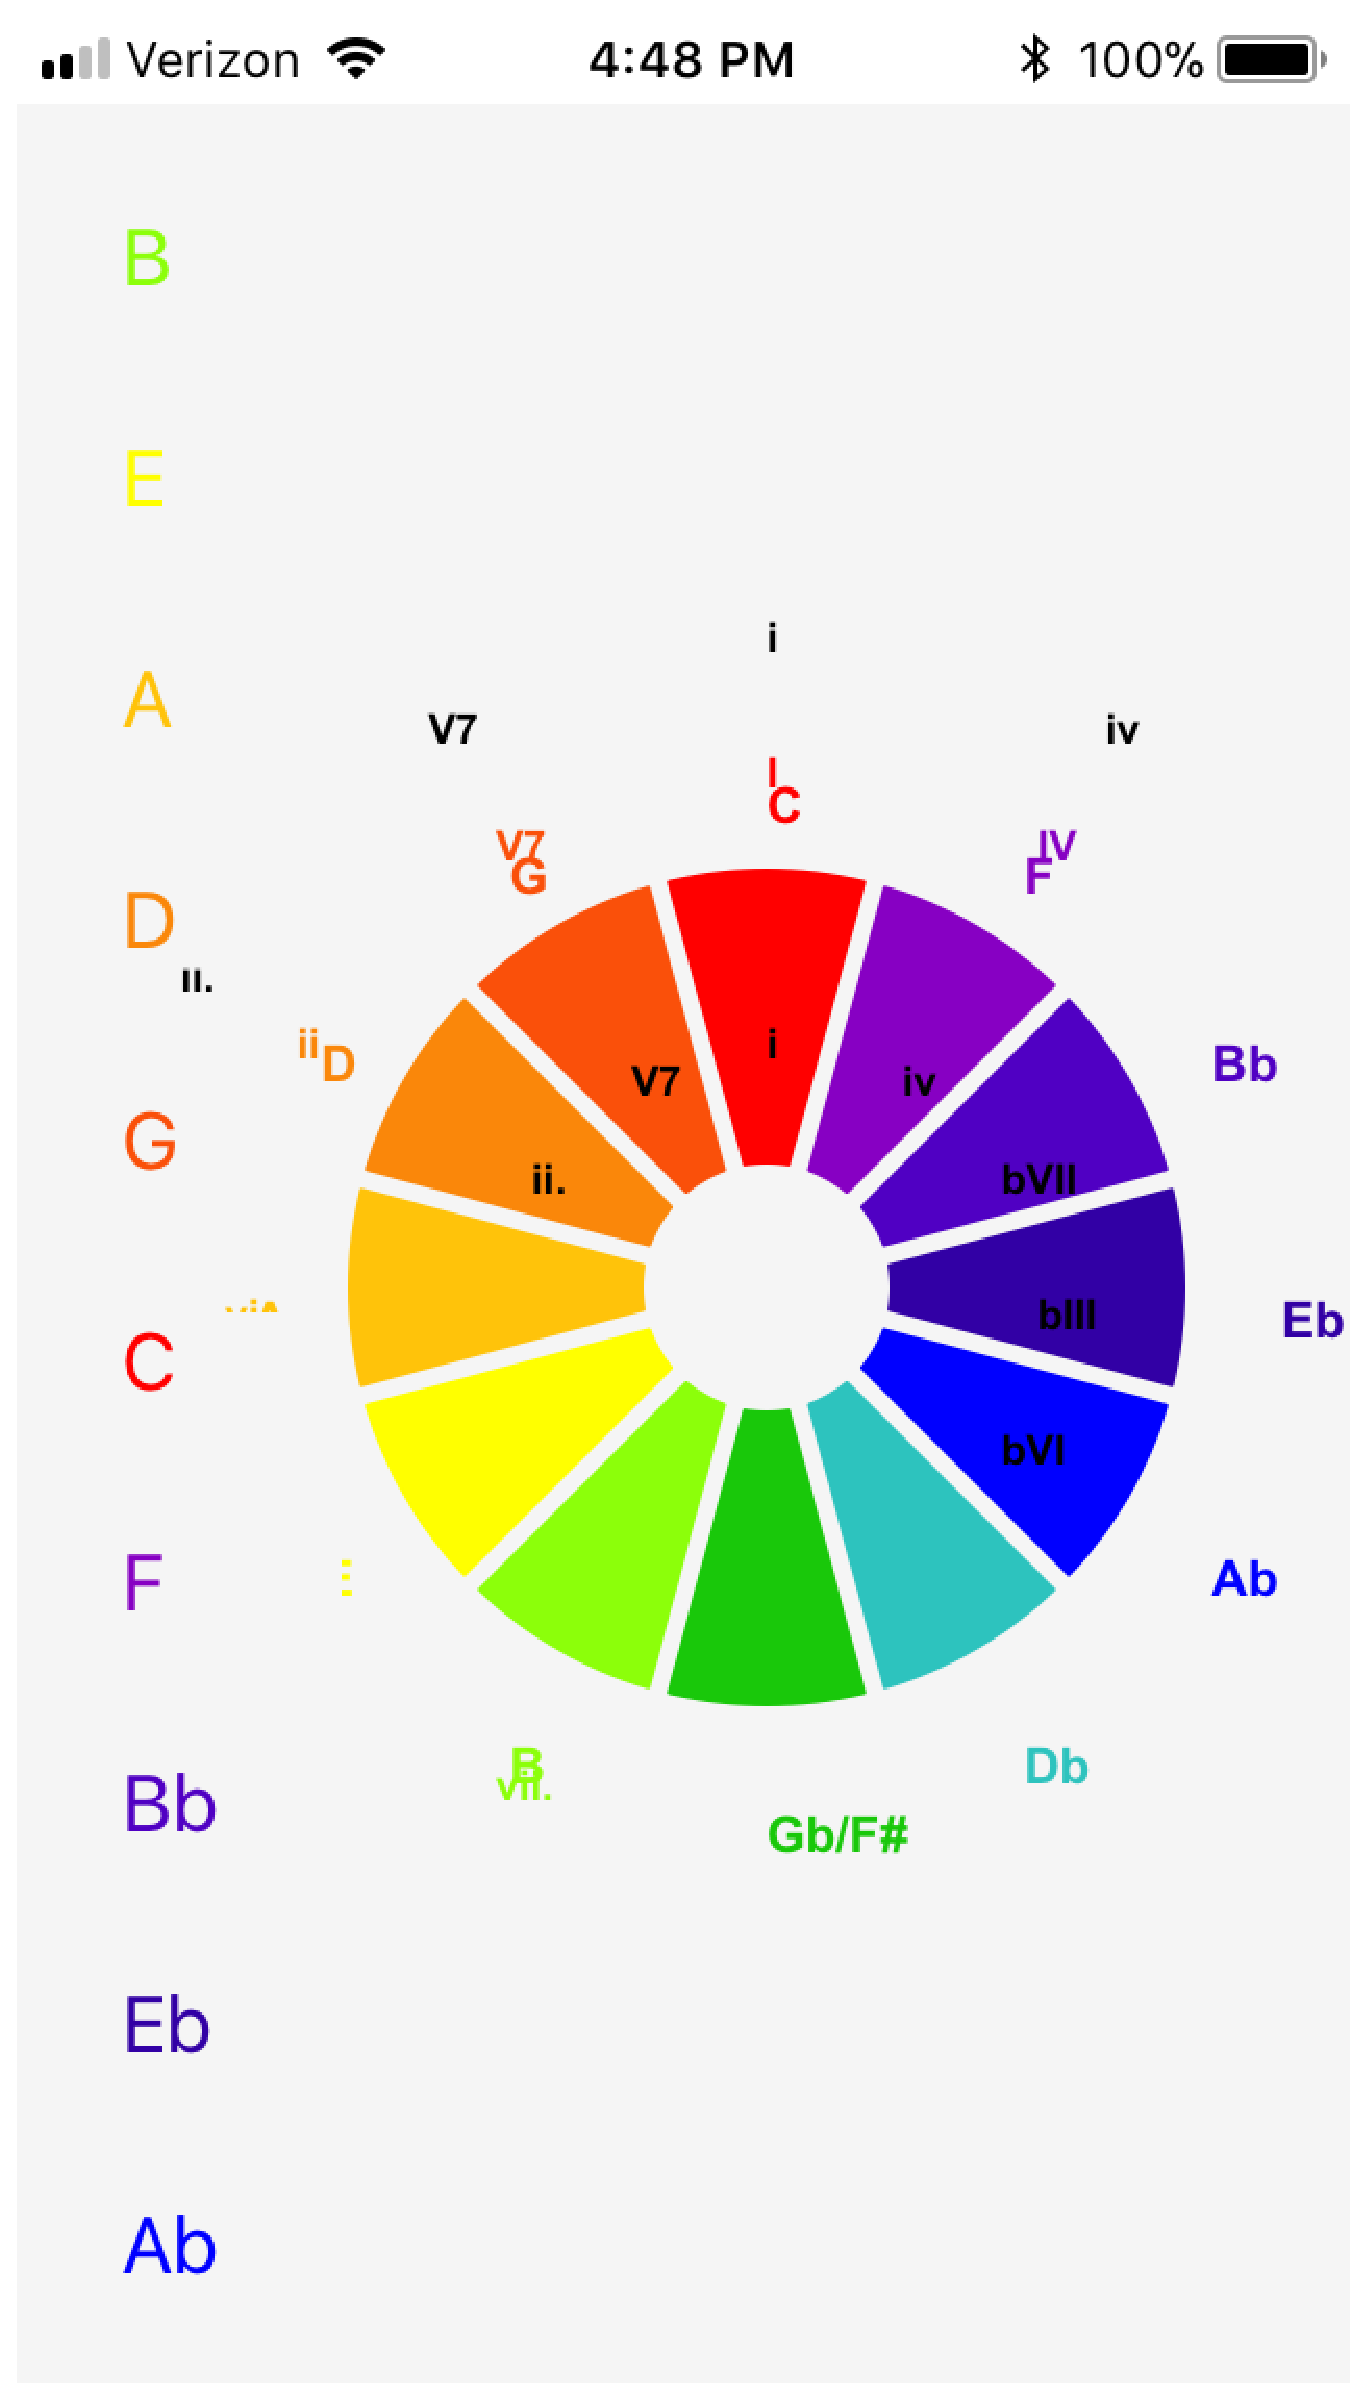
\includegraphics[width=5cm]{cof.eps}
\end{figure}

\paragraph{Implementation Design}
From an implementation viewpoint, using a vector based graphic that is drawn within the application is the implementation we have decided on for the Circle of Fifths.
There are many positives in using a graphic that is actually created within the application's source code.
he main positive being we have more customizability over the animations and interactions with the circle.
Since it is vector based, there will be no issues with resizing the graphic if necessary.
There are also a lot of different options for creating vector based graphics in React Native.
We will be creating the COF using the third party javascript libraries ART and d3 such as what is done in the article written by David Vacca to create a pie chart \cite{medium}.
We will use React’s built in Text component as well as the ART Text components to create the notes and chord qualities that are involved in the circle and will use basic circle geometry to place these components \cite{react-text} \cite{seb}.
We will use React’s PanResponder and Transform properties upon the circle to rotate the circle when the user gestures a spin \cite{react-pan} \cite{react-transforms}.
With these libraries and React Native components we will be able to achieve all of what the client has deemed necessary for the COF.

\paragraph{Rationale}
The rationale behind the design specified is to provide the user with a functioning and interactive circle of fifths that is also aesthitically pleasing and is relatively easy to develop.
Since the circle is used for most of the concepts being taught and since it is where most of the interactive learning will be implemented, the COF must be included in the application.

\subsubsection{Sidebar}
The sidebar is a critical piece of our application as it displays the schedule of tonal gravity for the current key to the user.
It consists of the 12 notes in western music in a vertical list.

\paragraph{GUI design}
From a design viewpoint, the UI design for the sidebar is a vertical list of the 12 notes of western music.
The colors of the notes will correspond to the colors of the notes on the actual COF.
This is necessary to provide consistency across the application.
The notes will be separated far enough apart for the average user to be able to select a specific note easily.
The notes of the current key will be highlighted.
Below is an image giving some idea of this design.

\begin{figure}[H]
  \centering
  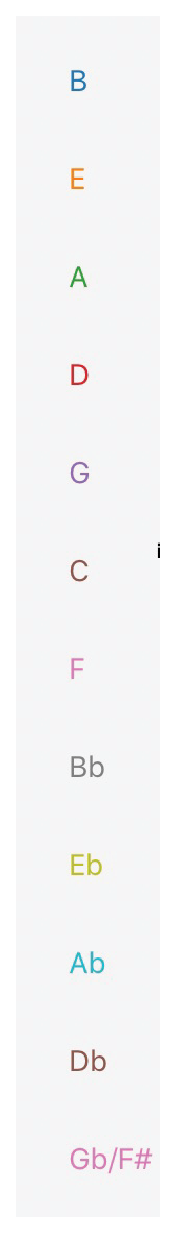
\includegraphics[height=7cm]{sidebar.eps}
\end{figure}

\paragraph{Implementation Design}
From an implementation viewpoint, the sidebar on our main Circle of Fifths page will combine both touching and dragging gestures to manipulate the contents of the COF.
Touching a specific note will bring that note to the top of the circle and reflect that note’s key.
Dragging along the length of the bar will bring whichever note the user’s finger is currently over to the top of the circle and that note’s major key will be reflected.
The main positive of this implementation is that users will be able to have options for altering the circle's contents and can end up focusing on one specific implementation based on personal preference.
If one user's fingers are too big to click the notes, they have the option to drag the bar.
If one user likes the dragging animation more than clicking then they can drag.
If a user likes to see their changes reflected on the circle immediately they can click a note.
Users need to be able to be comfortable with our app and giving options on how to use the app would be a big help in achieving comfort.
The implementation will be accomplished using React’s Text component to place the notes on the screen \cite{react-text}.
We will then use React’s PanResponder to implement responses to the user’s touching and dragging gestures;
the onPanResponderEnd function will signal a touch or the end of a drag and the onPanResponderMove function will signal a drag \cite{react-pan}.
This implementation will allow us to meet all of the goals we have outlined for this piece.
	
\paragraph{Rationale}
The sidebar is necessary for a completed application to help users understand the schedule of tonal gravity and to give users another way of manipulating the COF contents.
The implementation specified is necessary to give the user a few options of utilizing the sidebar to their preference.
	
\subsubsection{Buttons}
There will need to be multiple buttons on the Circle of Fifths page for adding parallel and relative keys as well as for navigating to different pages within the application.

\paragraph{Implementation Design}
Buttons within the Circle of Fifths page will be implemented with the React Native Button component \cite{react-button}.
The Button component comes with an onClick property which will be used to tell the application what should happen at this point.
If we are adding/removing keys to the COF we will just use the onClick property to call a function which will show/hide the specific key’s section on the page.
If we are changing screens we will use the React Native Navigator component to tell the application to navigate to the specific View we are navigating to \cite{react-navigators}.

\paragraph{Rationale}
The rationale behind the design specified above is that we need buttons to be able to let the user interact with different components of our application and to be able to change pages. 
There isn’t another way of implementing this functionality without the design specified for the buttons above.

\subsection{Composition Page}
\subsubsection{Chord Entry}

\begin{figure}[H]
    \centering
    \includegraphics[width=5cm]{entry.eps}
\end{figure}

\paragraph{GUI Design}
The circle of fifths style chord entry uses a circle of fifths for tone entry, as well as two groups of radio buttons for chord quality and 7th interval quality. 
The user will be able to touch any of the notes on the circle of fifths to determine the root tone of the chord.
The chord quality radio buttons are major, minor, or diminished.
The 7th interval quality radio buttons are none (n o 7th), 7th, major 7th, or diminished 7th.
The chord as it is entered will be displayed in the center.

\paragraph{Implementation Design}
A React Image Component will be used to implement the circle.
A Text Component will be used to implement the display for the chord being entered.
This will be updated when it receives events that come from the radio buttons.
The note buttons will be implemented using Button Components which set the state of the entered chord.
The other groups of radio buttons will be implemented using HTML Radio Input tags, which will also set the state of the entered chord.

\paragraph{Rationale}
The COF method of chord entry has very high cohesion with the another component of the app: the Circle of Fifths page.
This would allow users to develop muscle and spatial memory of the COF as they practice composing.

Implementing the COF style chord entry solves the problem simply and effectively, has the added benefit of drilling muscle memory for users, and has high cohesion with other parts of the app.

\subsubsection{Analysis}

\begin{figure}[H]
    \centering
    \includegraphics[width=5cm]{analysis.eps}
\end{figure}

\paragraph{GUI Design}
From this viewpoint, the user can push a button that will analyze or re-analyze the entire composition.
This element has 3 sub-elements: the current composition, the results, and the analyze button.
The current composition is made up of a “Composition” React Text Component, followed by another Text Component that contains the composition that has been entered so far.
The results is made up of a “Results:” Text Component, followed by a series of Text Components representing the results of the last analysis that was run.
Finally, the “Analyze” Button Component will re-analyze the composition when the user presses it.

\paragraph{Implementation Design}
In order to analyze the composition, the chords, their qualities, and their 7th qualities all need to be stored.
These can be stored as a record of note name, quality, and 7th quality.
The composition then can be stored as an ordered list of chords.
The Composition Text Component can be updated to reflect this ordered list, every time a new chord is added.

When the analyze button is pressed, a function will be mapped over each pair of chords in the ordered list which will determine if the transition from one chord to the next is acceptable according to the rules of tonal gravity.
The results will be collected.
A result should be a record of two chords, and the number of the rule that was broken.

\paragraph{Rationale}
A single analyze button was chosen since it is easy for the user to understand, without forcing analysis on the user.
This gives the user flexibility to ignore analysis if they feel like breaking the rules of tonal gravity.

\subsection{Reference Pages}
\begin{figure}[H]
    \centering
    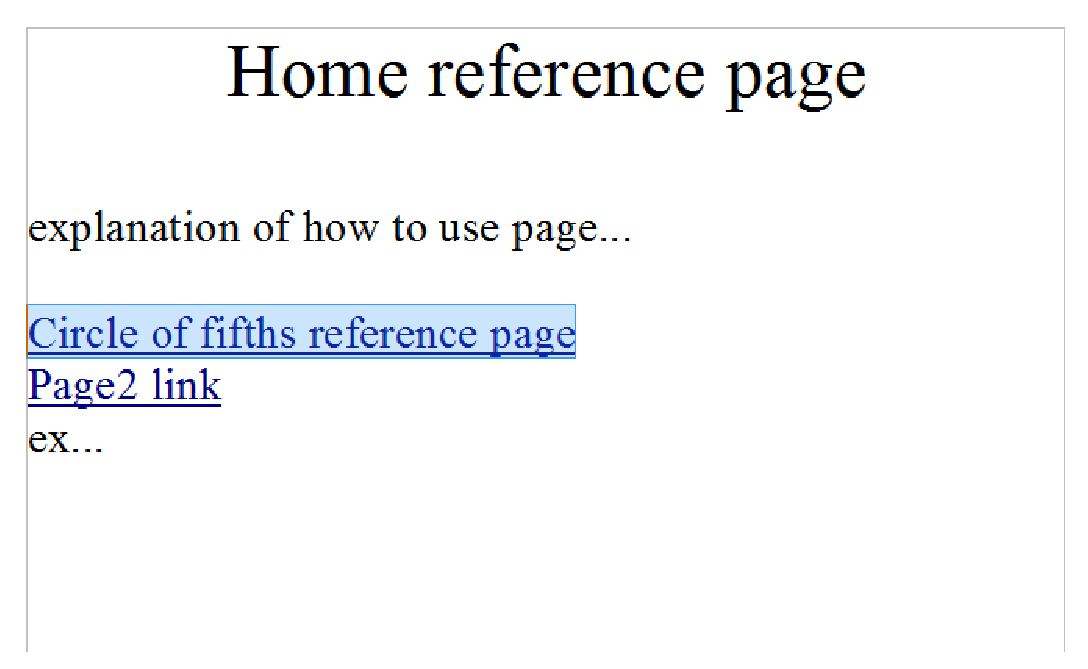
\includegraphics[width=5cm]{references.eps}
\end{figure}

\subsubsection{Implementation Design}
The implementation for these reference pages will be created using the React Native text component which the component for the reference page will contain.
The container component will utilize the React native (tabbed pages) component to contain the list of pages along with the pages themselves to easily navigate through.
This component will allow us to switch between different use cases of the application by listening for an onClick event, much like switching between tabs on a browser.
Once selected it will switch the view from the tab previously selected (either the circle of fifths tab or the composition/ comprehension tab), to the home page of the reference pages.
Here it will then display a list of links to the actual pages that describe and explain the different topics used within the application.
The main page will also contain a brief description of what can be found on each page and how to go about finding the information the user may be looking for. 

As a stretch goal we have also considered linking to these reference pages directly from the aspects of our application that might be explained by a specific reference page.
For instance when selected in a certain manner, the circle of fifths may display a pop-up dialogue box that gives a link to the circle of fifth’s reference page.
Another option would be allowing the pop-up itself to display the specific information a user might find helpful based on what they were clicking.

\subsubsection{Rationale}
Of the other options we considered, we decided that using reference pages would be the cleanest looking option.
Although this choice might make it slightly difficult to find the description of the topic the user may need assistance with, we decided it would still be the best option as it would allow us to provide any amount of information regarding a specific topic.
This would allow us to create more complete topic explanations and descriptions as we would not need to worry about providing too much or too little data that might confuse the user when compared to placing the references within the alternative options we considered.

%\bibliography{capstone}
%\bibliographystyle{IEEEtran}

\begin{thebibliography}{9}

\bibitem{medium}
  \textit{Animated Charts in React Native using D3 and ART}
  \\\texttt{{https://medium.com/the-react-native-log/animated-charts-in-react-native-using-d3-and-art-21cd9ccf6c58}}

\bibitem{react-transforms}
  \textit {Transforms}
  \\\texttt {{https://facebook.github.io/react-native/docs/transforms.html}}


\bibitem{react-navigators}
  \textit {Navigators}
  \\\texttt {{https://facebook.github.io/react-native/docs/navigators.html}}

\bibitem{react-image}
  \textit {Images}
  \\\texttt {{https://facebook.github.io/react-native/docs/image.html}}

\bibitem{react-text}
  \textit {Text}
  \\\texttt {{https://facebook.github.io/react-native/docs/text.html}}

\bibitem{react-view}
  \textit {View}
  \\\texttt {{https://facebook.github.io/react-native/docs/view.html}}

\bibitem{react-pan}
  \textit {PanResponder}
  \\\texttt {{https://facebook.github.io/react-native/docs/panresponder.html}}

\bibitem{react-button}
  \textit {PanResponder}
  \\\texttt {{https://facebook.github.io/react-native/docs/button.html}}

\bibitem{seb}
  \textit {ART.Text}
  \\\texttt {{http://sebmarkbage.github.io/art/docs/Shapes/ART.Text.html}}

\bibitem{omt-keysig}
  \textit {Key Signatures}
  \\\texttt {{http://openmusictheory.com/keySignatures.html}}

\bibitem{omt-intervals}
  \textit {Intervals}
  \\\texttt {{http://openmusictheory.com/intervals.html}}

\bibitem{omt-triads}
  \textit {Triads}
  \\\texttt {{http://openmusictheory.com/triads.html}}

\end{thebibliography}

\end{document}
